% !TEX root = ../main.tex
%

\section{Results}
\label{sec:results}


\subsection{Main findings}

\paragraph{\ac{LLM} moderators significantly improve synthetic discussions.} As is shown in Fig.~\ref{fig:toxicity_aq_stats}, comments in unmoderated discussions exhibit significantly worse toxicity and \ac{AQ} (ANOVA $p<.000$).\footnote{The large size and balanced nature of our dataset allows the use of parametric tests.} Both effects \emph{amplify over time} under all strategies when compared to unmoderated discussions, indicating a limited, but consistent restraining effect caused by the \ac{LLM} moderators over time (Table~\ref{tab:timeseries}).

\paragraph{Sophisticated facilitation strategies do not meaningfully further improve synthetic discussions.} The impact of the ``Rules Only'', ``Moderation'' and ``Facilitation Guidelines'' strategies is marginal, and sometimes even non-statistically significant compared to the second baseline (``No Instructions'') (Fig.~\ref{fig:toxicity_aq_stats}). This suggests that out-of-the-box \acp{LLM} may lack a high “skill ceiling” which would enable them to effectively use these advanced instructions. Alternatively, our experimental setup might not allow \acp{LLM} to show existing, advanced moderation skills, although previous research has demonstrated important limitations in \ac{LLM} moderators \cite{cho-etal-2024-language}. Even so, our study would suggest that these abilities, if existing, would be hard to observe or inconsistent under test conditions.

\paragraph{\ac{LLM} moderators intervene far too frequently.} Fig.~\ref{fig:intervention_count} demonstrates that \ac{LLM} moderators intervene at almost any opportunity. Additionally, \ac{LLM} user-agents exhibit atypical tolerance for excessive moderator interventions, whereas with human participants such repeated interventions often provoke irritation and increased toxicity \cite{schaffner_community_guidelines, make_reddit_great, proactive_moderation, cresci_pesonalized_interventions}.

\paragraph{Mistral and Qwen generate discussions more aligned with human diversity scores, despite being significantly smaller than the LLaMa model.} As is shown in Fig.~\ref{fig:rougel_model}, Qwen demonstrated the highest diversity among the evaluated models, indicating limited participant interaction (Section~\ref{ssec:methodology:diversity}), followed by Mistral Nemo and LLaMa. However, none of the models closely matched the diversity observed in human discussions. Notably, Mistral produced the most human-like comment lengths (Fig.~\ref{fig:comment_length_model}). LLaMa's lower diversity validates prior research suggesting that highly aligned \acp{LLM} struggle to replicate human  dynamics \cite{Park2023GenerativeAI, leng_2024}. Alternatively, it can also be attributed to its longer average comment length; we find that there is a statistically significant negative correlation between comment length and diversity in synthetic discussions ($p < .000$), although we can not verify this pattern in human-generated texts ($p = 0.775$). Despite these differences, the performance gaps among the models are relatively minor, although it is notable that smaller models, such as Mistral exhibit comparable potential to their larger counterparts (Qwen, LLaMa).

\paragraph{Finetuned instruction prompts are essential for eliciting toxic behavior in instruction-tuned \acp{LLM}.} Interactions involving “Troll” user-agents, directed by our finetuned instruction prompt, led to increased toxicity and decreased \ac{AQ} among other participants, even when moderated under the “No Instructions” strategy (Student's t-test, $p < .000$). This effect diminishes when explicit instructions\footnote{This comparison was conducted according to the ablation study setup presented in Section~\ref{ssec:results:ablation}.} to react to toxic posts are removed (Fig.~\ref{fig:boxplots}), with a similar, though less pronounced, impact on \ac{AQ}.

\begin{figure}[t]
    \centering
    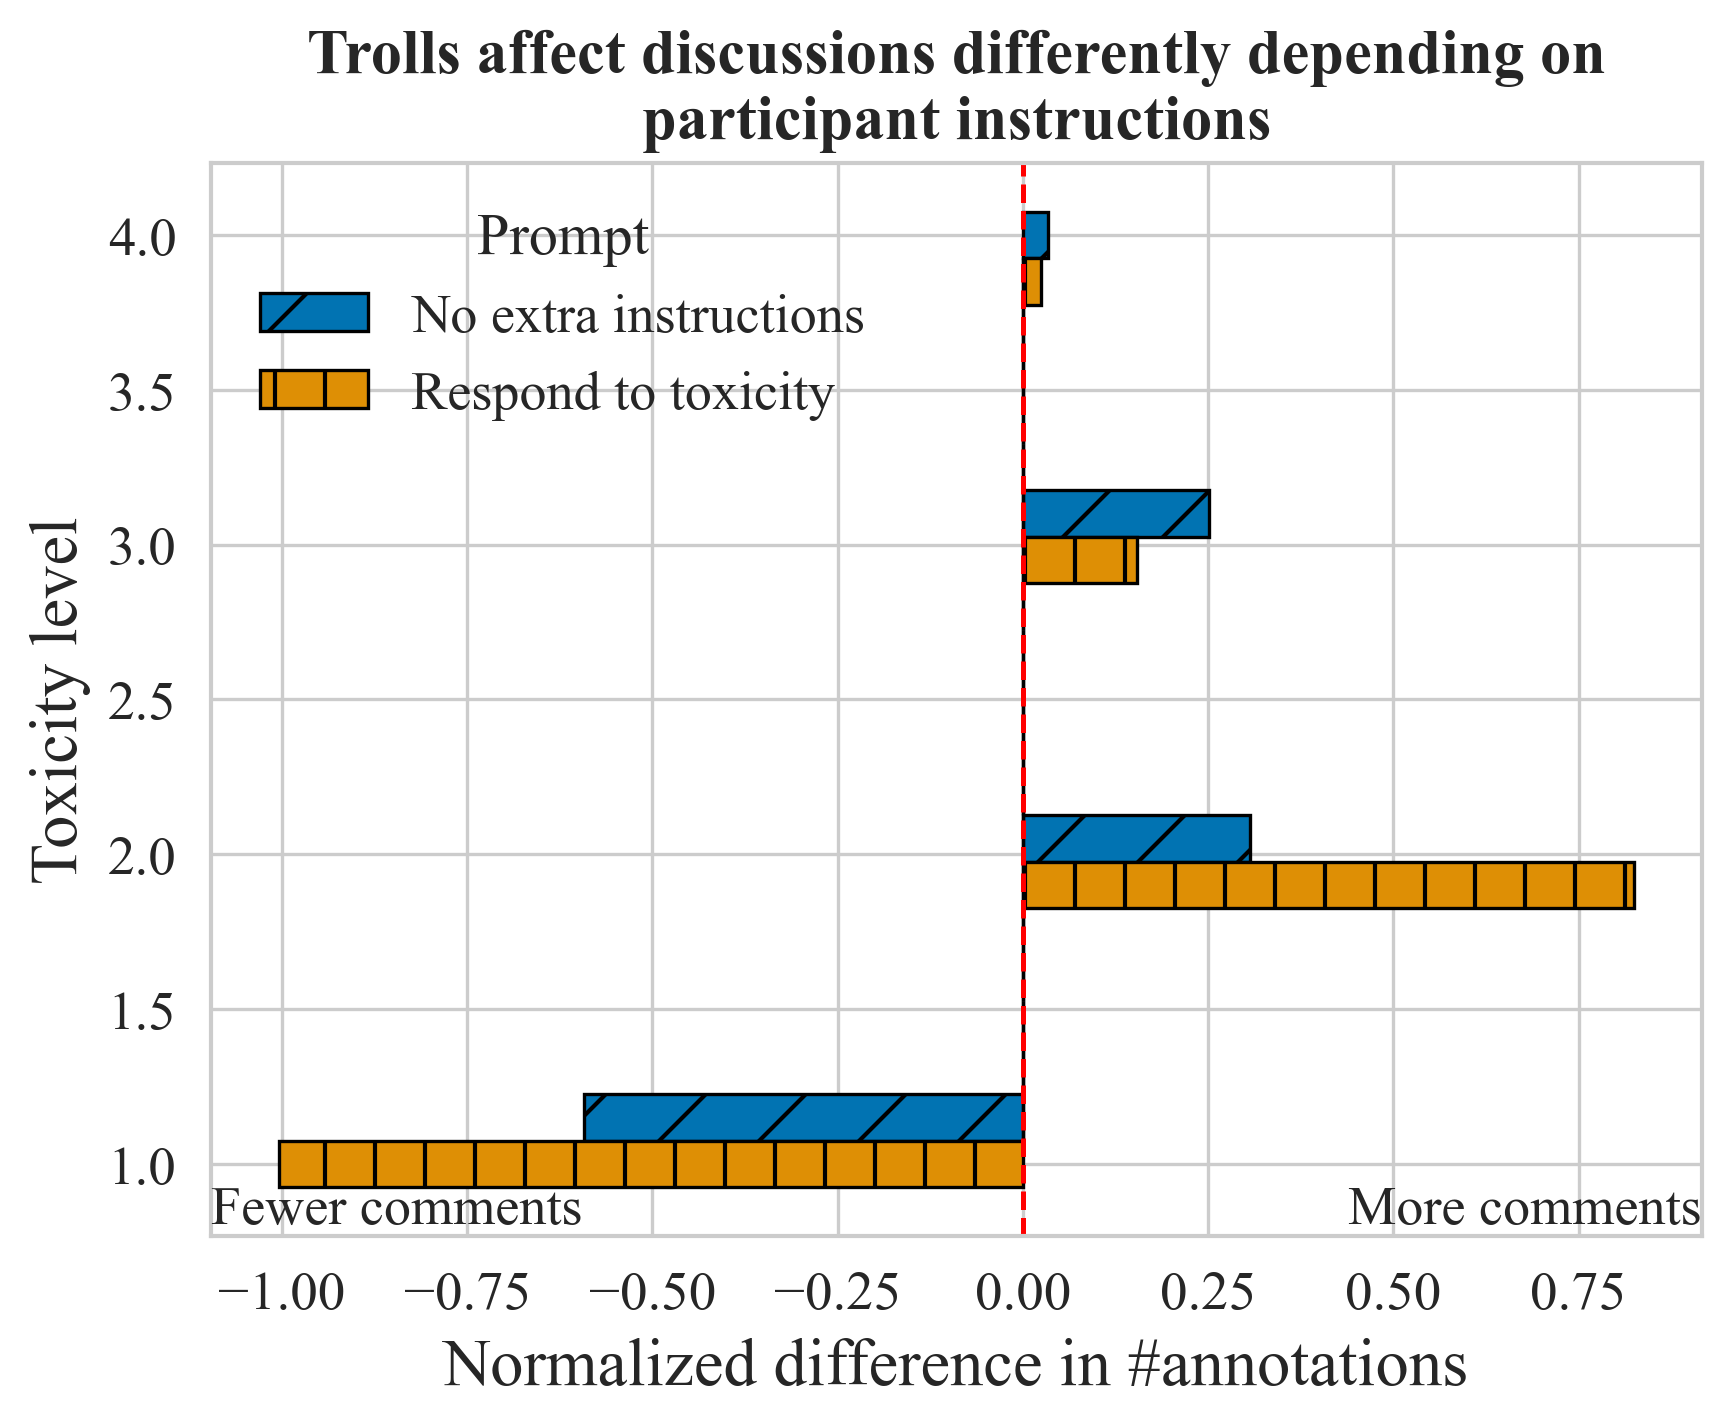
\includegraphics[width=0.49\linewidth]{toxicity_trolls.png} \hfill
    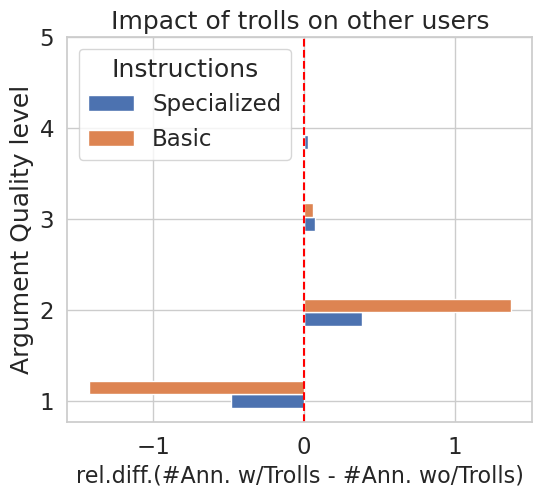
\includegraphics[width=0.49\linewidth]{aq_trolls.png}
    \caption{Relative differences in number of annotations by Toxicity (left) and \ac{AQ} (right) of synthetic discussions, excluding comments by troll user-agents. We compare between our original and a basic instruction prompt.}
    \label{fig:boxplots}
\end{figure}


\begin{figure}[t]
	\centering
	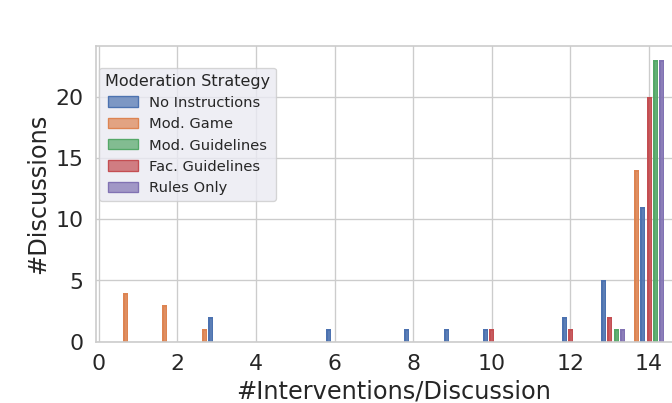
\includegraphics[width=\columnwidth]{intervention_count.png}
	\caption{Histogram of interventions by \ac{LLM} moderators. The maximum number of interventions is $14$.}
	\label{fig:intervention_count}
\end{figure}

\begin{figure*}[t]
    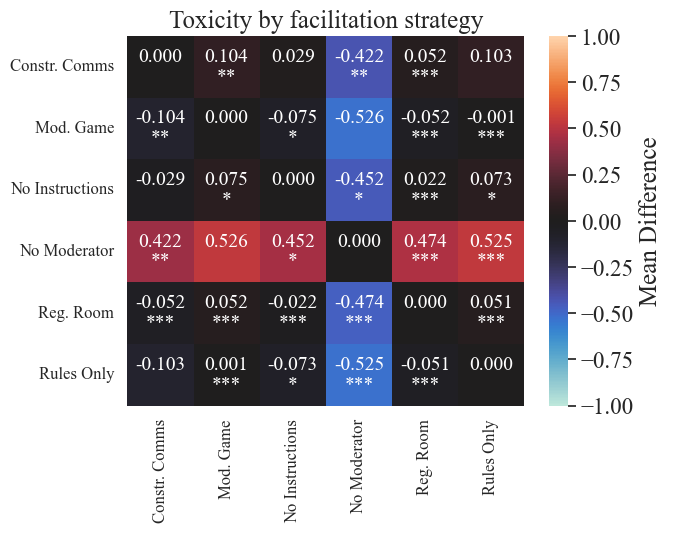
\includegraphics[width=0.49\linewidth]{toxicity_stats.png} \hfill
    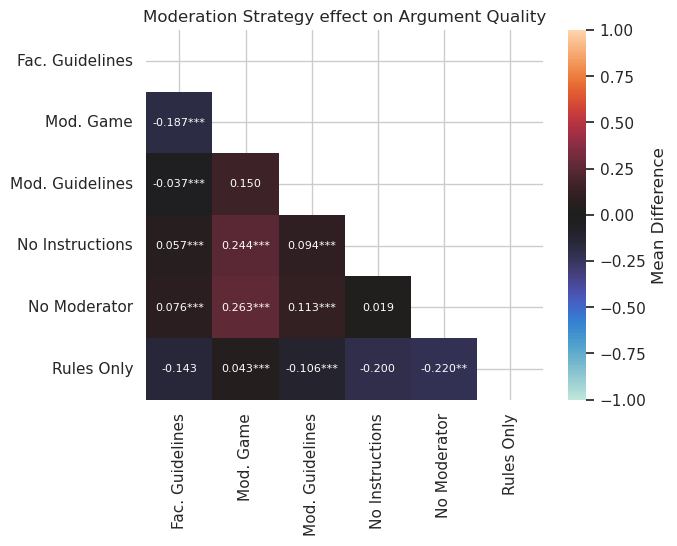
\includegraphics[width=0.49\linewidth]{argumentq_stats.png}
	\centering
	\caption{Mean difference of Toxicity (left) and \ac{AQ} (right) between each moderation strategy. $A[i, j] = 0.3^{***}$ indicates that the strategy $i$ leads to overall worse discussions (more toxicity/worse arguments) compared to $j$ for an average of $0.3$ annotation levels ($1-5$) with $p<.001$. Each comparison is accompanied by pairwise student-t tests, in the form of significance asterisks.}
	\label{fig:toxicity_aq_stats}
\end{figure*}

\begin{table}[t]
\centering
    \begin{tabular}{lll}
        \toprule
        \textbf{Variable} & \textbf{Toxicity} & \textbf{Arg.Q.} \\
        \midrule
        Intercept & 2.164\textsuperscript{***} & 2.113\textsuperscript{***} \\
        Fac. Guid. & -0.230\textsuperscript{***} & -0.007 \\
        Mod. Guid. & -0.277\textsuperscript{***} & -0.107\textsuperscript{*} \\
        \ac{RL} Game & -0.435\textsuperscript{***} & -0.282\textsuperscript{***} \\
        No Instructions & -0.426\textsuperscript{***} & -0.213\textsuperscript{***} \\
        Rules Only & -0.461\textsuperscript{***} & -0.305\textsuperscript{***} \\
        time & -0.012\textsuperscript{**} & -0.012\textsuperscript{**} \\
        Fac. Guid$\times$time & -0.023\textsuperscript{***} & -0.024\textsuperscript{***} \\
        Mod. Guid$\times$time & -0.023\textsuperscript{***} & -0.011\textsuperscript{*} \\
        \ac{RL} Game$\times$time & -0.011\textsuperscript{*} & 0.003 \\
        No Instructions$\times$time & -0.003 & 0.003 \\
        Rules Only$\times$time & -0.008 & -0.002 \\
        \bottomrule
    \end{tabular}
    \small
    $\cdot p<0.1$, \textsuperscript{*} $p<0.05$, \textsuperscript{**} $p<0.01$, \textsuperscript{***} $p<0.001$
    \normalsize
    \caption{OLS Regression Coefficients for Toxicity ($Adj. R^2=0.054$) and \ac{AQ} ($Adj. R^2=0.016$). \textit{“Time”} denotes dialogue turn, reference factor is \textit{“No moderator”}.}
    \label{tab:timeseries}
\end{table}



\subsection{Ablation study}
\label{ssec:results:ablation}

\begin{figure*}[t]
    \begin{subfigure}{0.32\linewidth}
        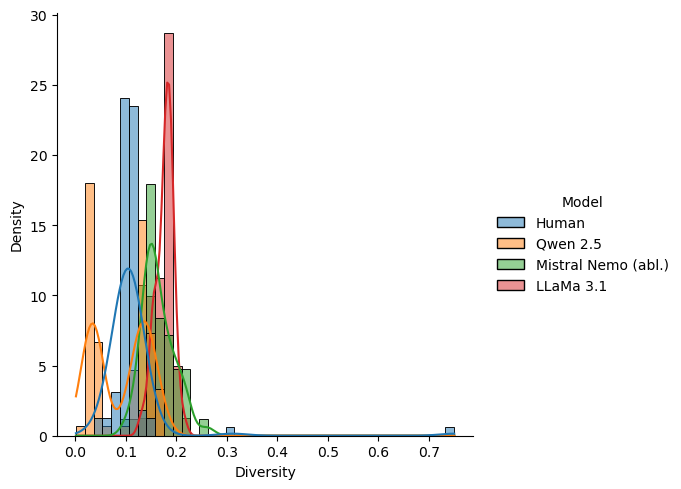
\includegraphics[width=\textwidth]{rougel_model.png}
        \caption{Model}
        \label{fig:rougel_model}
    \end{subfigure}%
    \hfill
    \begin{subfigure}{0.32\linewidth}
        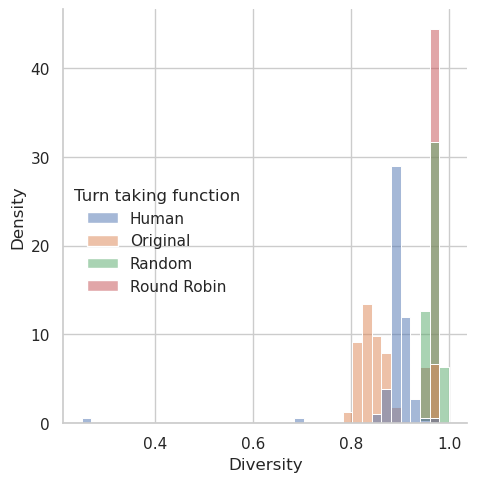
\includegraphics[width=\textwidth]{rougel_turns.png}
        \caption{Turn-taking function $t$}
        \label{fig:rougel_turns}
    \end{subfigure}%
    \hfill
    \begin{subfigure}{0.32\linewidth}
        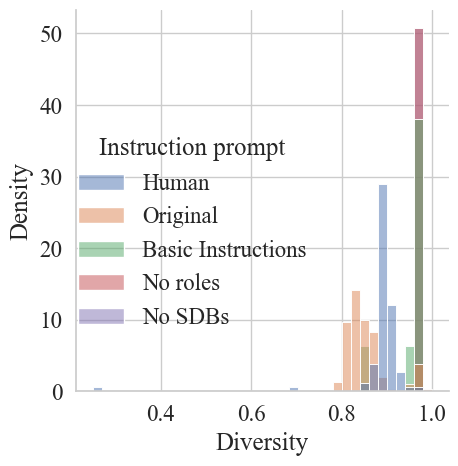
\includegraphics[width=\textwidth]{rougel_prompts.png}
        \caption{Promoting function $\phi$}
        \label{fig:rougel_prompts}
    \end{subfigure}%

    \caption{Diversity (Section~\ref{ssec:methodology:diversity}) distribution for each discussion by model (Section~\ref{ssec:experimental:setup}), turn-taking function $t$ (Section~\ref{ssec:experimental:turn}), and prompting function $\phi$ used (Section~\ref{ssec:experimental:prompts}).}
    \label{fig:diversity}
\end{figure*}

\begin{figure*}[t]
    \begin{subfigure}{0.32\linewidth}
        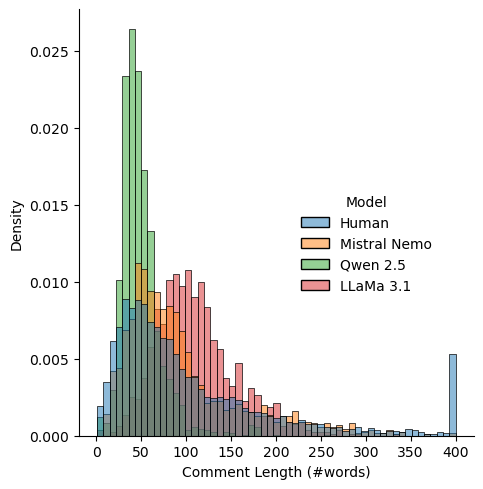
\includegraphics[width=\textwidth]{comment_len_model.png}
        \caption{Model}
        \label{fig:comment_length_model}
    \end{subfigure}%
    \hfill
    \begin{subfigure}{0.32\linewidth}
        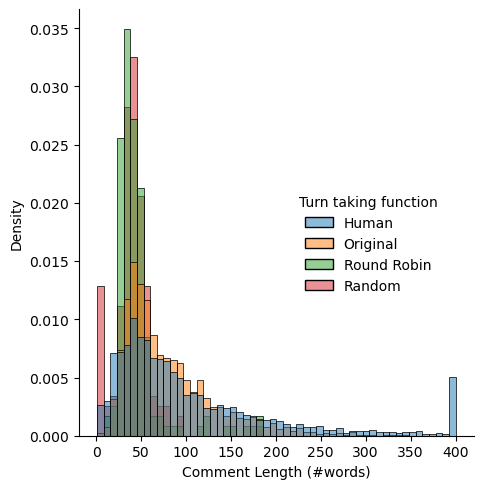
\includegraphics[width=\textwidth]{comment_len_turns.png}
        \caption{Turn-taking function $t$}
        \label{fig:comment_length_turns}
    \end{subfigure}%
    \hfill
    \begin{subfigure}{0.32\linewidth}
        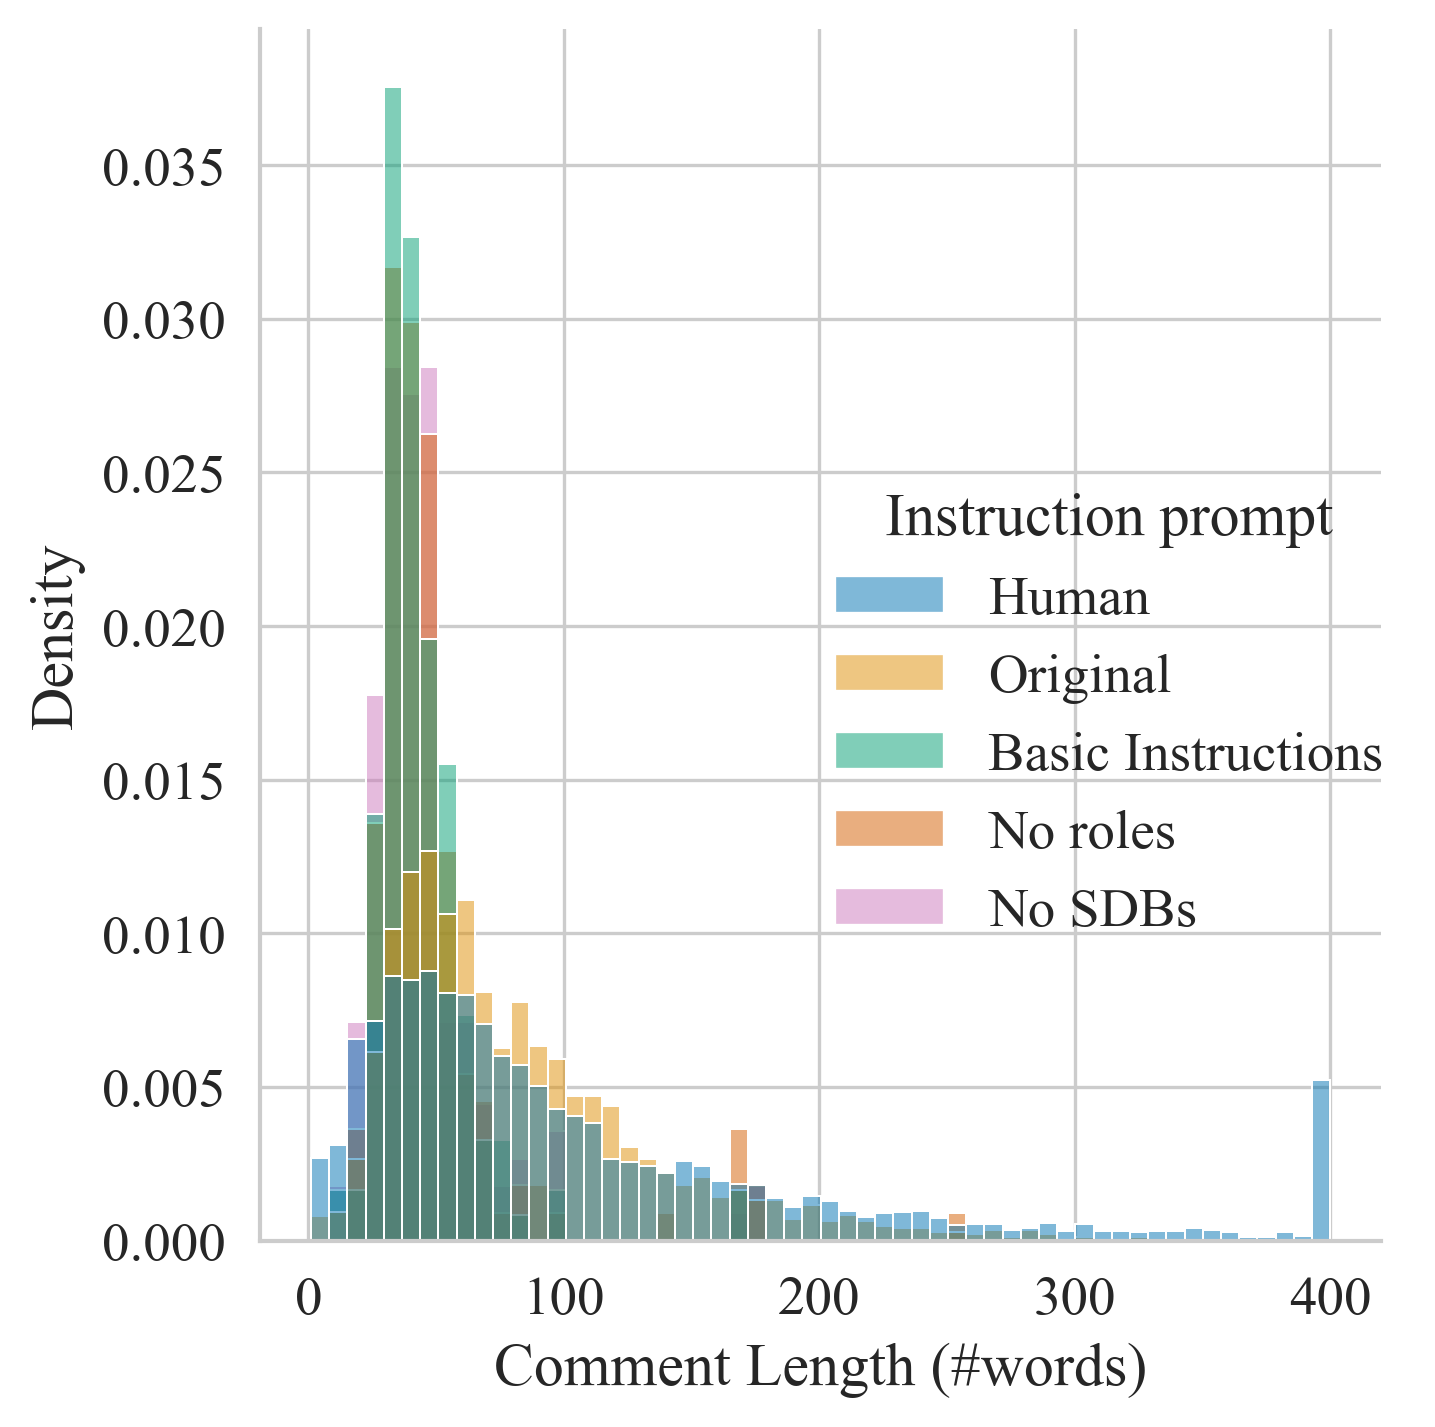
\includegraphics[width=\textwidth]{comment_len_prompts.png}
        \caption{Promoting function $\phi$}
        \label{fig:comment_length_prompts}
    \end{subfigure}%

    \caption{Comment length for each discussion by model (Section~\ref{ssec:experimental:setup}), turn-taking function $t$ (Section~\ref{ssec:experimental:turn}), and prompting function $\phi$ used (Section~\ref{ssec:experimental:prompts}). For ease of comparison, comments above 400 words are marked at the end of the x-axis.}
    \label{fig:comment_length}
\end{figure*}


In order to assess the impact of each component of our proposed methodology, we conducted eight synthetic discussions using a single model, Qwen, to limit computational cost. We evaluated the diversity of these generated discussions by comparing their diversity scores (cf. Section~\ref{ssec:methodology:diversity}) with i) discussions in our original dataset produced solely by the Qwen model; and ii) human discussions from the \ac{CeRI} “Regulation Room” dataset\footnote{\url{http://archive.regulationroom.org} Any opinions, findings, and conclusions or recommendations expressed in this material are those of the author(s) and do not necessarily reflect the views of the \ac{CeRI}} which includes moderated online deliberative discussions for ten diverse topics.


\subsubsection{Effects of turn taking functions}

\paragraph{Our proposed turn-taking function meaningfully improves the quality of synthetic data.} We compare our turn-taking function (Section~\ref{ssec:experimental:turn}) to two baselines: Round Robin (placing each participant in a predetermined queue) and Random Selection. Fig.~\ref{fig:rougel_turns} demonstrates that no single function fully approximates human diversity scores (all distributions diverge from the blue—human—distribution). However, unlike our own function, both baselines feature extremely high diversity. Additionally, Fig.~\ref{fig:comment_length_turns} demonstrates that comments in discussions following our turn-taking function emulate the length of human discussions. This may have partially affected the diversity scores.


\subsubsection{Effects of user-agent prompting}

We conduct three separate experiments in which user-agents (excluding moderators) are subjected to one of the following conditions at a time: (1) no assigned \acp{SDB}, (2) no assigned roles, or (3) only a basic instruction prompt (\S\ref{sssec:appendix:actors}). 

\paragraph{\acp{SDB}, roles and our instruction prompt increase the quality of synthetic data.} Fi.~\ref{fig:rougel_prompts} illustrates that although our proposed methodology—incorporating \acp{SDB}, roles, and finetuned instruction prompts—does not achieve discussions with diversity scores comparable to human ones, eliminating any component of our prompting mechanisms results in a notable deterioration. For instance, omitting \acp{SDB} (denoted as ``No \acp{SDB}'' and represented by the red distribution) causes the majority of discussions to exhibit maximum diversity—one—indicating a significant loss in participant interaction. This decline is analogous to the effects observed when modifying the turn-taking function. Also similarly to the turn-taking ablation study, our proposed methodology features comments that best emulate observed human comment length (Fig.~\ref{fig:comment_length_prompts}).